\documentclass[12pt,a4paper]{article}
\usepackage[spanish]{babel}
\usepackage[utf8]{inputenc}

\usepackage[right=2cm,left=2cm,top=4cm,bottom=2cm,headsep=0.5cm,footskip=0.5cm]{geometry}
\usepackage{graphicx,subfigure}
\usepackage{amsmath,amssymb}
\usepackage{underscore}
\usepackage{fancyhdr}
\usepackage{array}
\usepackage{yhmath}

\graphicspath{ {img/} }

\pagestyle{fancy}
\fancyhf{}
\rhead{\textbf{Alberto Navalón Lillo}}
\lhead{\textit{Física y Química: Repaso 3.º ESO}}

\begin{document}

\subsubsection*{1. Escribe las siguientes cantidades en unidades del Sistema Internacional y en notación científica, utilizando el método de los factores de conversión. Después, ordena de menor a mayor las que correspondan a la misma magnitud.}

\begin{itemize}
	\item Radio de la tierra: \(6370 km \Rightarrow 6370 km \cdot \frac{1000 m}{1 km} = 6,37 \cdot 10^6 m\)
	\item Masa de un hipopótamo: \(1400kg\)
	\item Récord mundial de los 100 m: \(958cs \Rightarrow 958cs \cdot \frac{1s}{100cs} = 9,58 s\)
	\item Altura de Pau Gasol: \(215cm \Rightarrow 215cm \cdot \frac{1m}{100cm} = 2,15m\)
	\item Velocidad máxima del AVE: \(300\text{ km/h} \Rightarrow 300\text{km/h} \cdot \frac{1000m}{1km} \cdot \frac{1h}{3600s} = 83,\wideparen{3}\text{ m/s}\)
	\item Radio de un átomo de hidrógeno: \(52pm \Rightarrow 52pm \cdot \frac{1m}{10^{12}pm} = 5,2 \cdot 10^{-11}m\)
	\item Masa del monoplaza de Fernando Alonso: \(0,605\text{ tm (toneladas)} \Rightarrow 0,605tm \cdot \frac{1000kg}{1tm} = 605kg\)
	\item Tamaño del virus de la gripe: \(120nm \Rightarrow 120nm \cdot \frac{1m}{10^9nm} = 1,2 \cdot 10^{-7}m\)
	\item Densidad del agua del mar: \(1,13\text{ g/mL} \Rightarrow 1,13\text{ g/cm}^3 \cdot \frac{1kg}{1000g} \cdot \frac{10^6\text{cm}^3}{1\text{m}^3} = 1130\text{ kg/m}^3\)
	\item Velocidad de un caracol: \(0,9\text{ cm/s} \Rightarrow 0,9\text{ cm/s} \cdot \frac{1m}{100cm} = 0,009\text{ m/s}\)
	\item Densidad del aire de esta habitación: \(1,225\text{ g/L} \Rightarrow 1,225\text{ g/dm}^3 \cdot \frac{1kg}{1000g} \cdot \frac{10^3\text{dm}^3}{1\text{m}^3} = 1,225\text{ kg/m}^3\)
\end{itemize}

\noindent Masa (kg): \(605kg < 1400kg\)\\
Longitud (m): \(5,2 \cdot 10^{-11} m < 1,2 \cdot 10^{-7} m < 2,15 m < 6,37 \cdot 10^6 m\)\\
Tiempo (s): \(9,58 s\)\\
Velocidad (m/s): \(0,009\text{ m/s} < 83,\wideparen{3}\text{ m/s}\)\\
Densidad (\(\text{kg/m}^3\)): \(1,225\text{ kg/m}^3 < 1130\text{ kg/m}^3\)

\subsubsection*{2. Un gas encerrado en un recipiente cerrado está sometido a una presión de 750mmHg y una temperatura de 25ºC. Calcula cuál será su temperatura si aumentamos la presión a 5 atm. ¿Qué ley estás aplicando?}

\textbf{Datos}:
\begin{itemize}
	\item \(V = cte.\)
	\item \(p_1 = 750mmHg\)
	\item \(p_2 = 5 atm \Rightarrow 5 atm \cdot \frac{760mmHg}{1atm} = 3800mmHg\)
	\item \(T_1 = 25ºC \Rightarrow 25ºC + 273 = 298K\)
	\item \(T_2?\)
\end{itemize}

Ley de Gay-Lussac:

\[
	\frac{p_1}{T_1} = \frac{p_2}{T_2} \Rightarrow \frac{750mmHg}{298K} = \frac{3800mmHg}{T_2} \Rightarrow T_2 = \frac{3800mmHg}{750mmHg} \cdot 298K = 1509,8\wideparen{6}K\Rightarrow
\]
\[
	\Rightarrow 1509,8\wideparen{6}K - 273 = 1236,8\wideparen{6}ºC
\]

\textbf{Solución}: la temperatura del gas a 5atm será de \textbf{1236,8ºC}. Estamos haciendo uso de la Ley de Gay-Lussac, ya que el volumen es constante.

\subsubsection*{3. Mezclamos 5g de hidróxido de sodio (NaOH) con 105g de agua. Sabiendo que su densidad es de 1,02g/mL, calcula:}

\begin{itemize}
	\item Gramos de disolución.
	\item Concentración en \% en masa.
	\item Concentración en g/L (aplicar aquí la densidad para calcular el volumen).
\end{itemize}

\noindent Datos:
\begin{itemize}
	\item Masa de soluto: 5g.
	\item Masa de disolución \(5g+105g=110g\)
	\item Densidad de disolución: 1,02g/mL.
\end{itemize}

\[
	\text{\% masa} = \frac{\text{masa de soluto}}{\text{masa de disolución}} \cdot 100 \Rightarrow \text{\% masa} = \frac{5g}{110g} \cdot 100 = 4,\wideparen{54}\%
\]

\[
	\text{C (g/L)} = \frac{\text{masa de soluto}}{\text{volumen de disolución}} \Rightarrow \text{C (g/L)} = \frac{\frac{5g}{1,02\text{g/mL}}}{1000} \approx 4,9 \cdot 10^{-3}\text{ g/L}
\]

\noindent Masa de disolución (g): 110g.\\
Concentración en \% en masa: \(4,\wideparen{54}\%\)\\
Concentración en g/L: \(4,9 \cdot 10^{-3}\text{ g/L}\)

\pagebreak

\subsubsection*{4. Dibuja el esqueleto de la tabla periódica y sitúa los siguientes elementos: calcio, magnesio, hierro, cobre, cloro, cinc, carbono, azufre, plomo.}

\begin{figure}[h]
	\centering
	\subfigure[Fig. A.]{
		\label{fig:a}
		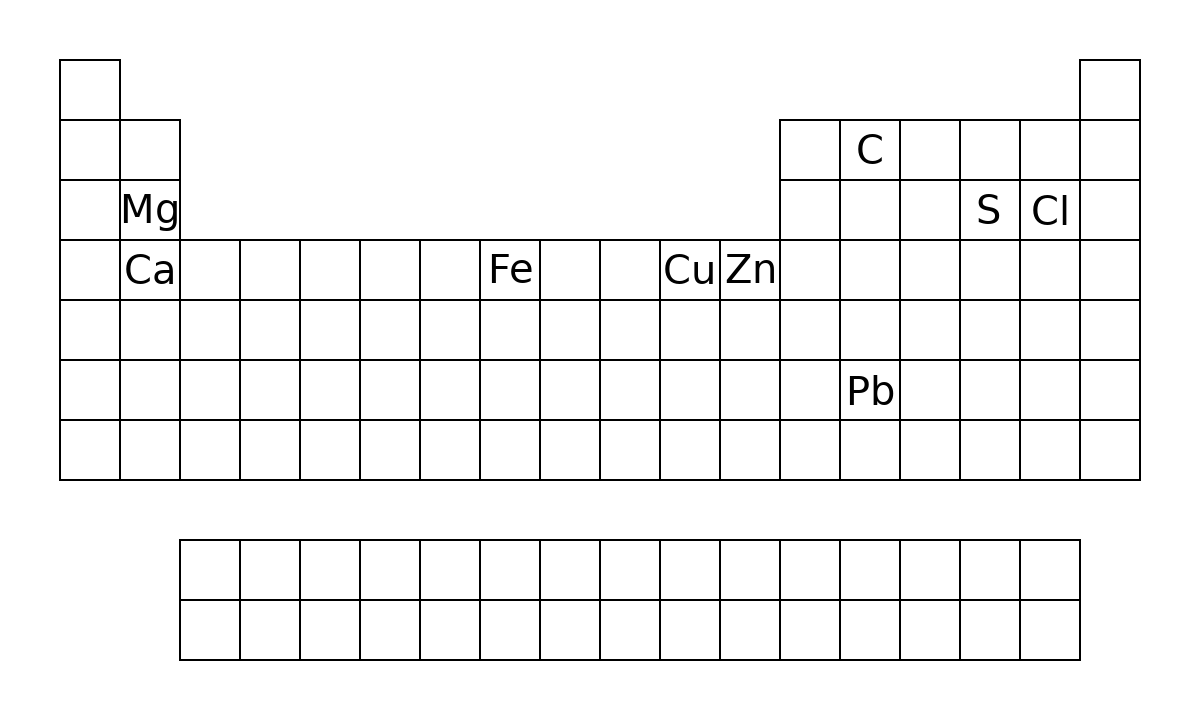
\includegraphics[width=15cm]{periodictable}
	}
\end{figure}

\subsubsection*{5. Escribe la configuración electrónica de los siguientes elementos buscando el número atómico en la tabla periódica: Na, Co, Ba, O, Cl, P, Ag, \(\text{Mg}^{2+}\text{, N}^{3-}\)}

\begin{itemize}
	\item Na (sodio): \(1s^2\text{ }2s^2\text{ }2p^4\text{ }3s^2\text{ }3p^1\)
	\item Co (cobalto): \(1s^2\text{ }2s^2\text{ }2p^4\text{ }3s^2\text{ }3p^4\text{ }4s^2\text{ }3d^10\text{ }4p^1\)
	\item Ba (bario): \(1s^2\text{ }2s^2\text{ }2p^4\text{ }3s^2\text{ }3p^4\text{ }4s^2\text{ }3d^10\text{ }4p^4\text{ }5s^2\text{ }4d^10\text{ }5p^4\text{ }6s^2\text{ }4f^8\)
	\item O (oxígeno): \(1s^2\text{ }2s^2\text{ }2p^4\)
	\item Cl (cloro): \(1s^2\text{ }2s^2\text{ }2p^4\text{ }3s^2\text{ }3p^4\text{ }4s^2\text{ }3d^1\)
	\item P (fósforo): \(1s^2\text{ }2s^2\text{ }2p^4\text{ }3s^2\text{ }3p^4\text{ }4s^1\)
	\item Ag (plata): \(1s^2\text{ }2s^2\text{ }2p^4\text{ }3s^2\text{ }3p^4\text{ }4s^2\text{ }3d^10\text{ }4p^4\text{ }5s^2\text{ }4d^10\text{ }5p^4\text{ }6s^1\)
	\item \(\text{Mg}^{2+}\) (magnesio): \(1s^2\text{ }2s^2\text{ }2p^4\text{ }3s^2\text{ }3p^4\text{ }4s^2\text{ }3d^7\)
	\item \(\text{N}^{3-}\) (nitrógeno): \(1s^2\text{ }2s^2\text{ }2p^4\text{ }3s^2\)
\end{itemize}

\subsubsection*{6a. Nombrar:}

\begin{itemize}
	\item \(Na_2O\): monóxido de disodio / óxido de sodio.
	\item \(ZnH_2\): dihidruro de cinc / hidruro de cinc.
	\item \(HCl\): cloruro de hidrógeno (ácido clorhídrico).
	\item \(NH_3\): trihidruro de nitrógeno / hidruro de nitrógeno(III) (azano o \textbf{amoniaco}).
	\item \(Fe_2O_3\): trióxido de dihierro / óxido de hierro(III).
	\item \(Cs_2O_2\): óxido de dicesio / peróxido de cesio.
\end{itemize}

\subsubsection*{6b. Formular:}

\begin{itemize}
	\item Hidruro de plata: \(AgH\)
	\item Sulfuro de hierro(III): \(Fe_2S_3\)
	\item Yoduro de hidrógeno: \(HI\)
	\item Metano: \(CH_4\)
	\item Trióxido de dinitrógeno: \(N_2O_3\)
	\item Peróxido de magnesio: \(MgO_2\)
\end{itemize}

\end{document}